

%%%%%%%%%%%%%%%%%%%%%%%%%%%%%%%%%%%%%%%%%%%%%%%%%%%%%%%
\subsubsection{Linear basis functions in tetrahedra ($P_1$)}
\index{general}{$P_1$}


\begin{verbatim}
(r_0,s_0) = (0,0,0)
(r_1,s_1) = (1,0,0)
(r_2,s_2) = (0,2,0)
(r_3,s_3) = (0,0,1)
\end{verbatim}

The basis polynomial is given by
\[
f(r,s,t)=c_0 + c_1 r + c_2 s + c_3 t
\]

\begin{eqnarray}
f_1 &=& f(r_1,s_1,t_1) = c_0 \\
f_2 &=& f(r_2,s_2,t_2) = c_0 + c_1\\
f_3 &=& f(r_3,s_3,t_3) = c_0 + c_2\\
f_4 &=& f(r_4,s_4,t_4) = c_0 + c_3
\end{eqnarray}

which yields:
\[
c_0=f_1
\quad
\quad
c_1=f_2-f_1
\quad
\quad
c_2=f_3-f_1
\quad
\quad
c_3=f_4-f_1
\]

\begin{eqnarray}
f(r,s,t) 
&=& c_0 + c_1 r + c_2 s + c_3 t \nonumber\\
&=& f_1 + (f_2-f_1) r + (f_3-f_1) s + (f_4-f_1) t \nonumber\\
&=& f_1 (1-r-s-t) + f_2 r + f_3 s + f_4 t \nonumber\\
&=& \sum_i N_i(r,s,t) f_i \nonumber
\end{eqnarray}

Finally,

\begin{mdframed}[backgroundcolor=blue!5]
\begin{eqnarray}
N_1(r,s,t) &=& 1-r-s-t \nonumber\\
N_2(r,s,t) &=& r \nonumber\\
N_3(r,s,t) &=& s \nonumber\\
N_4(r,s,t) &=& t \nonumber
\end{eqnarray}
\end{mdframed}

%%%%%%%%%%%%%%%%%%%%%%%%%%%%%%%%%%%%%%%%%%%%%%%%%%%%%%%
\subsubsection{Enriched linear in tetrahedra($P_1^+$)}
\index{general}{$P_1^+$}

These shape functions would be used in the MINI element, see Section~\ref{pair:mini}.

In 3D the buble function lools like $rst(1-r-s-t)$ so that 
\[
f(r,s,t)=a+b\; r+c\; s+d\; t+e \; rst(1-r-s-t)
\]
We have node 1 at location $(r,s,t)=(0,0,0)$, node 2 at $(r,s,t)=(1,0,0)$, node 3 at $(r,s,t)=(0,1,0)$ , 
node4 at $(r,s,t)=(0,0,1)$ and we 
set the location of the bubble (node 5) at $r=s=t=1/4$ so that 
\begin{eqnarray}
f(r_1,s_1,t_1)&=&f_1 = a+b\; r_1+c\; s_1+d\; t_1+e\; r_1s_1t_1(1-r_1-s_1-t_1) \\
f(r_2,s_2,t_2)&=&f_2 = a+b\; r_2+c\; s_2+d\; t_2+e\; r_2s_2t_2(1-r_2-s_2-t_2) \\
f(r_3,s_3,t_3)&=&f_3 = a+b\; r_3+c\; s_3+d\; t_3+e\; r_3s_3t_3(1-r_3-s_3-t_3) \\
f(r_4,s_4,t_4)&=&f_4 = a+b\; r_4+c\; s_4+d\; t_4+e\; r_4s_4t_4(1-r_4-s_4-t_4) \\ 
f(r_5,s_5,t_5)&=&f_5 = a+b\; r_5+c\; s_5+d\; t_5+e\; r_5s_5t_5(1-r_5-s_5-t_5) 
\end{eqnarray}
i.e.,
\begin{eqnarray}
f_1 &=& a\\
f_2 &=& a+b\\
f_3 &=& a+c\\
f_4 &=& a+d\\
f_5 &=& a+b/4+c/4+d/4+e/64 (1-1/4-1/4-1/4) \\ 
    &=& a+b/4+c/4+d/4+e/256  
\end{eqnarray}
Then 

\begin{eqnarray}
a&=&f_1\\
b&=&f_2-f_1\\
c&=&f_3-f_1\\
d&=&f_4-f_1\\
e&=&256(f_5-a-b/4-c/4-d/4) \\
&=&256(f_5-f_1-(f_2-f_1)/4-(f_3-f_1)/4-(f_4-f_1)/4) \\
&=&256(-f_1/4 - f_2/4 - f_3/4 - f_4/4 + f_5  ) \\
&=&64(-f_1 - f_2 - f_3 - f_4 + 4f_5  )
\end{eqnarray}
Finally:
\begin{eqnarray}
f(r,s,t)
&=& a+br+cs+dt+erst(1-r-s-t) \nn\\
&=& f_1 + (f_2-f_1)r + (f_3-f_1)s + (f_4-f_1)t+ 64(-f_1 - f_2 - f_3 - f_4 + 4f_5  ) rst(1-r-s-t)  \nn\\
&=& f_1 [1-r-s-t - 64rst(1-r-s-t)]\nn\\
&+& f_2 [r- 64rst(1-r-s-t)]\nn\\
&+& f_3 [s- 64rst(1-r-s-t)]\nn\\
&+& f_4 [t- 64rst(1-r-s-t)]\nn\\
&+& f_5 [256 rst(1-r-s-t)] \nn\\
&=&\sum_{i=1}^5 N_i(r,s,t) f_i
\end{eqnarray}
with
\begin{mdframed}[backgroundcolor=blue!5]
\begin{eqnarray}
N_1(r,s,t) &=& 1-r-s-t - 64rst(1-r-s-t) \\
N_2(r,s,t) &=& r - 64rst(1-r-s-t) \\
N_3(r,s,t) &=& s - 64rst(1-r-s-t) \\
N_4(r,s,t) &=& t - 64rst(1-r-s-t) \\
N_5(r,s,t) &=&  + 256rst(1-r-s-t) 
\end{eqnarray}
\end{mdframed}


%The question remains: in the papers about the MINI element, authors talk about adding the bubble function defined as
%$rs(1-r-s)$ in 2D but not about its coefficient. I am also curious about the isoparametric mapping. It seems to work, but would it be better/different with a simple P1 mapping?

The derivatives are given by:

\begin{eqnarray}
\frac{\partial N_1}{\partial r}(r,s,t) &=& -1 - 64st(1-2r-s-t) \nn\\
\frac{\partial N_2}{\partial r}(r,s,t) &=& +1 - 64st(1-2r-s-t) \nn\\
\frac{\partial N_3}{\partial r}(r,s,t) &=&    - 64st(1-2r-s-t) \nn\\
\frac{\partial N_4}{\partial r}(r,s,t) &=&    - 64st(1-2r-s-t) \nn\\
\frac{\partial N_5}{\partial r}(r,s,t) &=&     256st(1-2r-s-t) \nn\\ \nn\\ 
\frac{\partial N_1}{\partial s}(r,s,t) &=& -1 - 64rt(1-r-2s-t) \nn\\
\frac{\partial N_2}{\partial s}(r,s,t) &=&    - 64rt(1-r-2s-t) \nn\\
\frac{\partial N_3}{\partial s}(r,s,t) &=& +1 - 64rt(1-r-2s-t) \nn\\
\frac{\partial N_4}{\partial s}(r,s,t) &=&    - 64rt(1-r-2s-t) \nn\\
\frac{\partial N_5}{\partial s}(r,s,t) &=&     256rt(1-r-2s-t) \nn\\ \nn\\ 
\frac{\partial N_1}{\partial t}(r,s,t) &=& -1 - 64rs(1-r-s-2t) \nn\\
\frac{\partial N_2}{\partial t}(r,s,t) &=&    - 64rs(1-r-s-2t) \nn\\
\frac{\partial N_3}{\partial t}(r,s,t) &=&    - 64rs(1-r-s-2t) \nn\\
\frac{\partial N_4}{\partial t}(r,s,t) &=& +1 - 64rs(1-r-s-2t) \nn\\
\frac{\partial N_5}{\partial t}(r,s,t) &=&     256rs(1-r-s-2t) \nn
\end{eqnarray}






%%%%%%%%%%%%%%%%%%%%%%%%%%%%%%%%%%%%%%%%%%%%%%%%%%%%%%%
\subsubsection{Triquadratic basis functions in 3D ($Q_2$)}
\index{general}{$Q_2$}

\begin{verbatim}
   t
   |
   .--s
  /
 r
                                    05=====16=====08 
                                    |      |      |  
                                    |      |      |  
                  13=====26=====15  17=====25=====20 
                  |      |      |   |      |      |  
                  |      |      |   |      |      |  
06=====14=====07  22=====27=====24  01=====12=====04 @ r=-1
|      |      |   |      |      |  
|      |      |   |      |      |   
18=====23=====14  09=====21=====11 @ r=0
|      |      |   
|      |      |  
02=====10=====03 @ r=+1
\end{verbatim}





\begin{eqnarray}
N_{1}&=& 0.5r(r-1)  \;0.5s(s-1)\; 0.5t(t-1)  \nonumber\\
N_{2}&=& 0.5r(r+1)  \;0.5s(s-1)\; 0.5t(t-1)  \nonumber\\
N_{3}&=& 0.5r(r+1)  \;0.5s(s+1)\; 0.5t(t-1)  \nonumber\\
N_{4}&=& 0.5r(r-1)  \;0.5s(s+1)\; 0.5t(t-1)  \nonumber\\
N_{5}&=& 0.5r(r-1)  \;0.5s(s-1)\; 0.5t(t+1)  \nonumber\\
N_{6}&=& 0.5r(r+1)  \;0.5s(s-1)\; 0.5t(t+1)  \nonumber\\
N_{7}&=& 0.5r(r+1)  \;0.5s(s+1)\; 0.5t(t+1)  \nonumber\\
N_{8}&=& 0.5r(r-1)  \;0.5s(s+1)\; 0.5t(t+1)  \nonumber\\
N_{9}&=& (1-r^2)   \;0.5s(s-1)\; 0.5t(t-1)  \nonumber\\
N_{10}&=& 0.5r(r+1) \;(1-s^2)  \; 0.5t(t-1)  \nonumber\\
N_{11}&=& (1-r^2)  \;0.5s(s+1)\; 0.5t(t-1)  \nonumber\\
N_{12}&=& 0.5r(r-1) \;(1-s^2)  \; 0.5t(t-1)  \nonumber\\
N_{13}&=& (1-r^2)  \;0.5s(s-1)\; 0.5t(t+1)  \nonumber\\
N_{14}&=& 0.5r(r+1) \;(1-s^2)  \; 0.5t(t+1)  \nonumber\\
N_{15}&=& (1-r^2)  \;0.5s(s+1)\; 0.5t(t+1)  \nonumber\\
N_{16}&=& 0.5r(r-1) \;(1-s^2)  \; 0.5t(t+1)  \nonumber\\
N_{17}&=& 0.5r(r-1) \;0.5s(s-1)\; (1-t^2)  \nonumber\\
N_{18}&=& 0.5r(r+1) \;0.5s(s-1)\; (1-t^2)  \nonumber\\
N_{19}&=& 0.5r(r+1) \;0.5s(s+1)\; (1-t^2)  \nonumber\\
N_{20}&=& 0.5r(r-1) \;0.5s(s+1)\; (1-t^2)  \nonumber\\
N_{21}&=& (1-r^2)   \;(1-s^2)  \; 0.5t(t-1)  \nonumber\\
N_{22}&=& (1-r^2)   \;0.5s(s-1)\; (1-t^2)  \nonumber\\
N_{23}&=& 0.5r(r+1) \;(1-s^2)  \; (1-t^2)  \nonumber\\
N_{24}&=& (1-r^2)   \;0.5s(s+1)\; (1-t^2)  \nonumber\\
N_{25}&=& 0.5r(r-1) \;(1-s^2)  \; (1-t^2)  \nonumber\\
N_{26}&=& (1-r^2)   \;(1-s^2)  \; 0.5t(t+1)  \nonumber\\
N_{27}&=& (1-r^2)   \;(1-s^2)  \; (1-t^2)  \nonumber
\end{eqnarray}

%.....................................................................
\subsubsection{Enriched quadratic basis functions in tetrahedra ($P_2^+$)}
\index{general}{$P_2^+$}

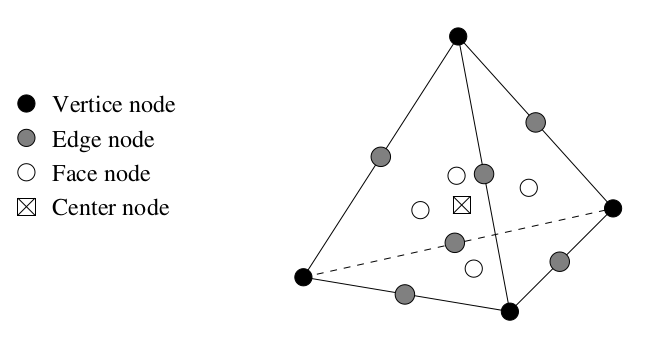
\includegraphics[width=9cm]{images/crouzeix-raviart/p2pp1_3D1}
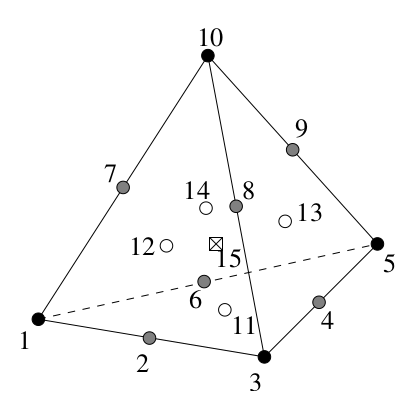
\includegraphics[width=5cm]{images/crouzeix-raviart/p2pp1_3D2}

The velocity shape functions are:
\begin{eqnarray}
\phi_i &=& \lambda_i(2\lambda_i-1) + 3 (\lambda_i\lambda_j \lambda_k + \lambda_i\lambda_j\lambda_l + \lambda_i\lambda_k\lambda_l) -4 \lambda_i\lambda_j\lambda_k\lambda_l \\
\phi_{ij} &=& 4\lambda_i\lambda_j - 12( \lambda_i\lambda_j\lambda_k+\lambda_i\lambda_j\lambda_l  ) +32 \lambda_i\lambda_j\lambda_k \lambda_l \\
\phi_{ijk} &=& 27  \lambda_i\lambda_j\lambda_k - 108 \lambda_i\lambda_j\lambda_k \lambda_l \\
\phi_c &=& 256 \lambda_i\lambda_j\lambda_k\lambda_l
\end{eqnarray}

\todo[inline]{REFS ??? better definition of functions !}

%.....................................................................
\subsubsection{Linear basis functions for tetrahedra ($P_1$)}
\index{general}{$P_1$}

This is essentially in the $Q_2\times P_{-1}$ element. 

I choose the reduced coordinates of the pressure nodes to be :

\begin{tabular}{cccc}
\hline
point & r & s & t \\
\hline
1& 1/2 &-1/2 &-1/2\\
2& -1/2 &1/2 &-1/2\\
3& -1/2 &-1/2& 1/2\\
4& 1/2 &1/2& 1/2 \\
\hline
\end{tabular}

Inside the element the pressure is given as a linear function of the reduced coordinates $r,s,t$:
\[
p(r,s,t)=a+br+cs+dt
\]
This expression must exactly interpolate the pressure at all four pressure nodes:
\begin{eqnarray}
p_1 
&=& p(r_1,s_1,t_1) 
= a+br_1+cs_1+dt_1 
= a+b/2-c/2-d/2\nonumber\\
p_2
&=& p(r_2,s_2,t_2)
= a+br_2+cs_2+dt_2
= a-b/2+c/2-d/2\nonumber\\
p_3
&=& p(r_3,s_3,t_3) 
= a+br_3+cs_3+dt_3 
= a-b/2-c/2+d/2\nonumber\\
p_4
&=& p(r_4,s_4,t_4) 
= a+br_4+cs_4+dt_4
= a+b/2+c/2+d/2\nonumber
\end{eqnarray}
or,
\begin{equation}
\left(
\begin{array}{cccc}
1 & 1/2 & -1/2 & -1/2 \\
1 & -1/2 & +1/2 & -1/2 \\
1 & -1/2 & -1/2 & +1/2 \\
1 & 1/2 & +1/2 & +1/2 
\end{array}
\right)
\left(
\begin{array}{c}
a\\b\\c\\d
\end{array}
\right)=
\left(
\begin{array}{c}
p_1\\p_2\\p_3\\p_4
\end{array}
\right)
\nonumber
\end{equation}

The matrix is invertible and we get:
\[
\left(
\begin{array}{c}
a\\b\\c\\d
\end{array}
\right)=
\left(
\begin{array}{cccc}
1/4 & 1/4 & 1/4 & 1/4 \\
1/2 & -1/2 & -1/2 & 1/2 \\
-1/2 & 1/2 & -1/2 & 1/2 \\
-1/2 & -1/2 & 1/2 & 1/2
\end{array}
\right)
\left(
\begin{array}{c}
p_1\\p_2\\p_3\\p_4
\end{array}
\right)
\]

so 
\begin{eqnarray}
p(r,s,t)
&=& a+br+cs+dt \nonumber\\
&=& \frac{1}{4}(p_1+p_2+p_3+p_4)
+\frac{1}{2}(p_1-p_2-p_3+p_4)r
+\frac{1}{2}(-p_1+p_2-p_3+p_4)s
+\frac{1}{2}(-p_1-p_2+p_3+p_4)t\nonumber\\
&=&
\frac{1}{4}(1+2r-2s-2t)p_1+
\frac{1}{4}(1-2r+2s-2t)p_2+
\frac{1}{4}(1-2r-2s+2t)p_3+
\frac{1}{4}(1+2r+2s+2t)p_4 \nonumber\\
&=& \sum_{i=1}^4 N_i(r,s,t) p_i
\end{eqnarray}
with
\begin{eqnarray}
N_1(r,s,t) &=& \frac{1}{4}(1+2r-2s-2t)\nonumber\\
N_2(r,s,t) &=& \frac{1}{4}(1-2r+2s-2t)\nonumber\\
N_3(r,s,t) &=& \frac{1}{4}(1-2r-2s+2t)\nonumber\\
N_4(r,s,t) &=& \frac{1}{4}(1+2r+2s+2t)\nonumber
\end{eqnarray}

%%%%%%%%%%%%%%%%%%%%%%%%%%%%%%%%%%%%%%%%%%%%%%%%%%%%%%%%%%%%%%%%%%%%%
\subsubsection{20-node serendipity basis functions in 3D ($Q_2^{(20)}$)}
\index{general}{$Q_2^{(20)}$} \index{general}{Serendipity element}

The serendipity elements are those rectangular elements which have no
interior nodes \cite[p91]{reddybook2}.

\begin{verbatim}
   t
   |
   .--s
  /
 r
                                    05=====20=====08 
                                    |             |  
                                    |             |  
                  17 - - - - - -19  13            16
                  .              .  |             |  
                  .              .  |             |  
06=====18=====07  .              .  01=====12=====04 @ r=-1
|             |   .              . 
|             |   .              .  
14            15  09 - - - - - -11 @ r=0
|             |   
|             |  
02=====10=====03 @ r=+1
\end{verbatim}

\todo[inline]{find/build shape functions!}


%..........................................................................---------------------------
\subsubsection{Enriched linear basis functions in quadrilaterals ($Q_1^+$) -WIP} \label{ss:quadmini3D}
\index{general}{$Q_1^+$}

Following Lamichhane (2017) \cite{lami17} we can define two bubble functions to enrich the 
$Q_1$ space:

\begin{eqnarray}
b^{(1)} (r,s,t) &=& (1-r)(1-s)(1-t) \cdot (1-r^2) (1-s^2) (1-t^2) \\
b^{(2)} (r,s,t) &=& (1 + \beta(r+s+t)) \cdot (1-r^2) (1-s^2) (1-t^2) 
\end{eqnarray}

The first one includes a tri-linear term while the second one includes a linear one parameterised by $\beta$.
In both cases the bubble is identically zero on the edges of the reference element and it is exactly 1 
in its middle.

\begin{eqnarray}
\frac{\partial b^{(1)}}{\partial r}(r,s,t) &=& (3r^2-2r-1)(1-y)(1-y^2)(1-t)(1-t^2) \\ 
\frac{\partial b^{(1)}}{\partial s}(r,s,t) &=& (3s^2-2s-1)(1-r)(1-r^2)(1-t)(1-t^2) \\ 
\frac{\partial b^{(1)}}{\partial t}(r,s,t) &=& (3t^2-2t-1)(1-r)(1-r^2)(1-s)(1-s^2)  
\end{eqnarray}

\begin{eqnarray}
\frac{\partial b^{(2)}}{\partial r}(r,s,t) &=&  -[b(3r^2+2r(s+t)-1)+2r](1-s^2)(1-t^2)\\
\frac{\partial b^{(2)}}{\partial s}(r,s,t) &=&  -[b(3s^2+2s(r+t)-1)+2s](1-r^2)(1-t^2)\\
\frac{\partial b^{(2)}}{\partial t}(r,s,t) &=&  -[b(3t^2+2t(r+s)-1)+2t](1-r^2)(1-s^2)
\end{eqnarray}












